%%%%%%%%%%%%%%%%%%%%%%%%%%%%%%%%%%%%%%%%%
% Beamer Presentation
% LaTeX Template
% Version 1.0 (10/11/12)
%
% This template has been downloaded from:
% http://www.LaTeXTemplates.com
%
% License:
% CC BY-NC-SA 3.0 (http://creativecommons.org/licenses/by-nc-sa/3.0/)
%
%%%%%%%%%%%%%%%%%%%%%%%%%%%%%%%%%%%%%%%%%

%----------------------------------------------------------------------------------------
%	PACKAGES AND THEMES
%----------------------------------------------------------------------------------------

\documentclass{beamer}
\usepackage{pgfpages}
\usepackage{avant}
%\setbeameroption{show notes}
%\setbeameroption{show notes on second screen=right}


\mode<presentation> {

% The Beamer class comes with a number of default slide themes
% which change the colors and layouts of slides. Below this is a list
% of all the themes, uncomment each in turn to see what they look like.

%\usetheme{default}
%\usetheme{AnnArbor}
%\usetheme{Antibes}
%\usetheme{Bergen}
%\usetheme{Berkeley}
%\usetheme{Berlin}
%\usetheme{Boadilla}
%\usetheme{CambridgeUS}
%\usetheme{Copenhagen}
%\usetheme{Darmstadt}
%\usetheme{Dresden}
%\usetheme{Frankfurt}
%\usetheme{Goettingen}
%\usetheme{Hannover}
%\usetheme{Ilmenau}
%\usetheme{JuanLesPins}
%\usetheme{Luebeck}
\usetheme{Madrid}
%\usetheme{Malmoe}
%\usetheme{Marburg}
%\usetheme{Montpellier}
%\usetheme{PaloAlto}
%\usetheme{Pittsburgh}
%\usetheme{Rochester}
%\usetheme{Singapore}
%\usetheme{Szeged}
%\usetheme{Warsaw}

% As well as themes, the Beamer class has a number of color themes
% for any slide theme. Uncomment each of these in turn to see how it
% changes the colors of your current slide theme.

%\usecolortheme{albatross}
%\usecolortheme{beaver}
%\usecolortheme{beetle}
%\usecolortheme{crane}
\usecolortheme{dolphin}
%\usecolortheme{dove}
%\usecolortheme{fly}
%\usecolortheme{lily}
%\usecolortheme{orchid}
%\usecolortheme{rose}
%\usecolortheme{seagull}
%\usecolortheme{seahorse}
%\usecolortheme{whale}
%\usecolortheme{wolverine}

%\setbeamertemplate{footline} % To remove the footer line in all slides uncomment this line
%\setbeamertemplate{footline}[1] % To replace the footer line in all slides with a simple slide count uncomment this line

\setbeamertemplate{navigation symbols}{} % To remove the navigation symbols from the bottom of all slides uncomment this line
}


\usepackage{graphicx} % Allows including images
\usepackage{booktabs} % Allows the use of \toprule, \midrule and \bottomrule in tables

\usepackage{animate}
\usepackage{transparent}
\usepackage{color}
\usepackage{tikz}
\usepackage[absolute,overlay]{textpos}

\definecolor{isrocol}{RGB}{1, 162, 216}

\setbeamercolor{block title}{bg=isrocol,fg=white}


%code snippets

\usepackage{listings} % Required for inserting code snippets
 % Required for specifying custom colors and referring to colors by name

\definecolor{DarkGreen}{rgb}{0.0,0.4,0.0} % Comment color
\definecolor{highlight}{RGB}{190,190,190} % Code highlight color

\lstdefinestyle{Style1}{ % Define a style for your code snippet, multiple definitions can be made if, for example, you wish to insert multiple code snippets using different programming languages into one document
language=bash, % Detects keywords, comments, strings, functions, etc for the language specified
backgroundcolor=\color{highlight}, % Set the background color for the snippet - useful for highlighting
basicstyle=\footnotesize\ttfamily, % The default font size and style of the code
breakatwhitespace=false, % If true, only allows line breaks at white space
breaklines=true, % Automatic line breaking (prevents code from protruding outside the box)
captionpos=b, % Sets the caption position: b for bottom; t for top
commentstyle=\usefont{T1}{pcr}{m}{sl}\color{DarkGreen}, % Style of comments within the code - dark green courier font
deletekeywords={}, % If you want to delete any keywords from the current language separate them by commas
%escapeinside={\%}, % This allows you to escape to LaTeX using the character in the bracket
firstnumber=1, % Line numbers begin at line 1
frame=single, % Frame around the code box, value can be: none, leftline, topline, bottomline, lines, single, shadowbox
frameround=tttt, % Rounds the corners of the frame for the top left, top right, bottom left and bottom right positions
keywordstyle=\color{Blue}\bf, % Functions are bold and blue
morekeywords={}, % Add any functions no included by default here separated by commas
numbers=left, % Location of line numbers, can take the values of: none, left, right
numbersep=10pt, % Distance of line numbers from the code box
numberstyle=\tiny\color{Gray}, % Style used for line numbers
rulecolor=\color{black}, % Frame border color
showstringspaces=false, % Don't put marks in string spaces
showtabs=false, % Display tabs in the code as lines
stepnumber=5, % The step distance between line numbers, i.e. how often will lines be numbered
stringstyle=\color{Purple}, % Strings are purple
tabsize=2, % Number of spaces per tab in the code
}

% Create a command to cleanly insert a snippet with the style above anywhere in the document
\newcommand{\insertcode}[2]{\begin{itemize}\item[]\lstinputlisting[caption=#2,label=#1,style=Style1]{#1}\end{itemize}} % The first argument is the script location/filename and the second is a caption for the listing



%----------------------------------------------------------------------------------------
%	TITLE PAGE
%----------------------------------------------------------------------------------------

\title[Linux File System]{\color{white} \textbf{The Linux File System\\}} % The short title appears at the bottom of every slide, the full title is only on the title page
\subtitle{\color{white}3. Introduction to Scientific Computing with Linux\\Part I. Introduction}

 % Your name
\institute[FOSS-IIST] % Your institution as it will appear on the bottom of every slide, may be shorthand to save space
{

\begin{flushright}
\color{white}
{
B.Tech Aerospace Engineering\\
Indian Institute of Space Science and Technology} % Your institution for the title page

 \textit{\\gowtham.sc13b020@ug.iist.ac.in}
\\ 
 \end{flushright} % Your email address
}
 % Date, can be changed to a custom date
 \date{\color{white} {FOSS Club, IIST, 2016}}
\begin{document}
\renewcommand*\footnoterule{}


\newcommand\blfootnote[1]{%
  \begingroup
  \renewcommand\thefootnote{}\footnote{#1}%
  \addtocounter{footnote}{-1}%
  \endgroup
}


\usebackgroundtemplate%
{%
    
\includegraphics[width=\paperwidth,height=\paperheight]{linux_bg}%
}
 
{
\setbeamertemplate{footline}{} 
\begin{frame}

\vspace*{3.8cm}
\color{white}
\begin{flushright}
Gowtham S
\end{flushright}
\vspace{-4.5cm}

\titlepage % Print the title page as the first slide


	\end{frame}
}
\section*{Title and Outline}

\author{Gowtham S}

\addtocounter{framenumber}{-1}

 \usebackgroundtemplate{}

\begin{frame}
\frametitle{Outline}

\tableofcontents
\end{frame}

\section{Introduction}
\begin{frame}{What is File System?}

It has got two meanings, \blfootnote{This tutorial mainly focuses on the $1^{st}$ variation}

\begin{block}{Variation 1}
\begin{itemize}
\item[] $\diamond$ File System is the "directory" structure or the hierarchy of your system
\item[] $\diamond$ On Linux and Unix, it is referred to as directory tree
\end{itemize}

\end{block}
\pause
\begin{block}{Variation 2}
\begin{itemize}
\item[] $\diamond$ A method or the way the files are organized on the disk or a partition on harddisk
\item[] $\diamond$ Example :
   \begin{itemize}
   \item[] $\diamond$ FAT16, FAT32, NTFS
   \item[] $\diamond$ ext2, ext3, ext4
   \end{itemize}
\end{itemize}
\end{block}

\end{frame}

\begin{frame}{Filesystem Hierarchy Standard in Linux}

\begin{block}{To see the directory list}
Open up a terminal and type in
\insertcode{scripts/filesystem_hier.sh}{}
\centering
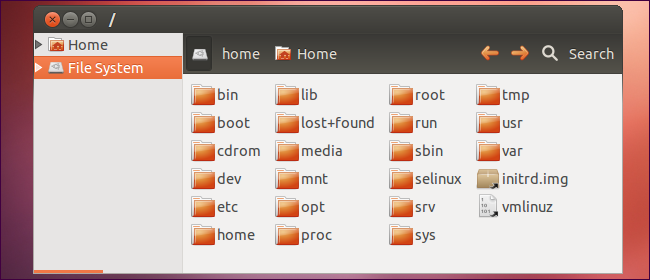
\includegraphics[scale=0.6]{filesystem_list}
\end{block}

\end{frame}

\section{Filesystem structure in Linux}
\subsection{/ - Root }

\begin{frame}{/ - The Root Directory}

\begin{itemize}
 \setlength\itemsep{0.8em}
\item <1-> EVERYTHING is nested under this directory
\item <2-> All other directories are `children' of this directory 
\item <3->  Similar to C:\textbackslash  on Windows (Note: Linux doesn't have drive letters)
\item <4-> Other partition appears in another folder in `/' on Linux (while D:\textbackslash on Windows)
\item <5-> The partition in which the root file system resides on is mounted first during boot 

\end{itemize}
\end{frame}

\subsection{/bin - User binaries}
\begin{frame}{/bin - Essential User Binaries}
\begin{itemize}
 \setlength\itemsep{0.8em}
\item <1-> Location for Ready-to-run programs 
\item <2-> bash shell is located here
\item <3-> Ensures availability of the most basic commands for the system
\begin{block}{/bin includes }
\begin{itemize}
\item[] $\diamond$ File manipulation tools (cat, cp, mv, rm, tar)
\item[] $\diamond$ Editors (vi, sed)
\item[] $\diamond$ File system tools (df, mount, umount)
\end{itemize}

\end{block}
\item <4-> Shared by the system with all the users
\end{itemize}
\end{frame}

\begin{frame}{/boot - Static files of bootloader}

\begin{itemize}
\setlength\itemsep{0.8em}
\item <1-> Location for image files required for the boot process
\item <2-> Kernel file (eg: vmlinuz-4.2.0) is stored here
\begin{block}{So what is the kernel?}
$\diamond$ Wiki: "The central core of the computer's OS"

\vspace{0.2cm}
$\diamond$ A software that interfaces with the hardware of your system

\vspace{0.2cm}
$\diamond$ Responsible for low-level tasks such as disk management, task management and memory management
\end{block}
\item <3-> /boot/grub contains GRUB (GNU GRand Unified Bootloader) 
\end{itemize}
\end{frame}

\subsection{/dev - Device files}
\begin{frame}{/dev - Essential device files}

\begin{itemize}
\setlength\itemsep{0.8em}
\item <1-> Everything is a file or a directory in Linux filesystem.
\item <2-> Every partition will appear as a file (eg: sda1, usb, dvd) in this directory
\item <3-> Contains references to all the hardware (represented as files) 
\item <4-> A device can be created using "makedev" script located here
\end{itemize}
\pause
\begin{block}{Some devices located in /dev}
\begin{itemize}
\item[] $\diamond$ /dev/usb (USB devices)
\item[] $\diamond$ /dev/dsp (AUDIO devices)
\item[] $\diamond$ /dev/sda (SCSI - HDD devices)
\end{itemize}
\end{block}
\end{frame}


\subsection{/etc - System Config}
\begin{frame}{/etc - Systemwide Configuration files}

\begin{itemize}
\item It is the Control panel (or) nerve center of your system
\pause
\item  etc is not etcetera directory. It is \textbf{E}ditable \textbf{T}ext \textbf{C}onfiguration or \textbf{E}xtended \textbf{T}ool \textbf{C}hest  \footnote{\url{www.blackmoreops.com/2015/06/18/linux-file-system-hierarchy-v2-0/}}
\end{itemize}
\pause
\begin{block}{Some of the contents of /etc}
\begin{itemize}
\item[] $\diamond$ /etc/bash.bashrc (System wide shell functions and aliases)
\item[] $\diamond$ /etc/X11 (X window system)
\item[] $\diamond$ /etc/apt (front-end dpkg package manager)
\item[] $\diamond$ /etc/dict.conf (Client for dictionary server)
\item[] $\diamond$ /etc/fstab (Config file for mount)
\end{itemize}

\end{block}
\end{frame}

\subsection{/home - User home directories}
\begin{frame}{/home - Home Sweet Home}

\begin{itemize}
\item Specific directory for each user which can be accessible only by the user and the SYSADMIN
\pause
\item Contains personal configuration files ("." files are hidden)
\insertcode{scripts/home_content.sh}{}
\item These personal configuration overrides the systemwide configuration
\end{itemize}

\begin{block}{Some important contens of /home}
\begin{itemize}
\item[] $\diamond$ /home/.bashrc Personal settings for the shell
\item[] $\diamond$ /home/.fonts Directory for personal fonts
\end{itemize}
\end{block}
\end{frame}

\begin{frame}{/root - Home of the root user}
Wait.. Is there a root on root?? 

\begin{itemize}
 \setlength\itemsep{0.8em}
 \item Note the difference between the `/' and `/root'
\item This is the administrator's home directory 
\pause
\vspace{0.3cm}
\begin{block}{Why not in /home itself?}
/home is often located in separate partition, this enables the sysadmin to access files even if the `/home' is not mounted
\end{block}
\end{itemize}
\end{frame}

\subsection{/lib - Library and Kernel modules}

\begin{frame}{/lib - Library files}
\begin{itemize}
\setlength\itemsep{0.8em}
\item Location of files for all kinds of programs needed by the system and the users
\item Essential files for basic system functionality
\pause
\item Similar to DLL files in Windows are located here
\end{itemize}

\begin{block}{Some of the contents}
\begin{itemize}
\item[] $\diamond$ C programming code library is located here
\item[] $\diamond$ /lib/x8$6\_6$4-linux-gnu/ (Contains platform/architecture dependent libraries)
\item[] $\diamond$ /lib/modules/ (Contains all kernal modules)
\end{itemize}
\end{block}

\end{frame}


\subsection{/media Mount point}

\begin{frame}{/media - Mount point}
\begin{itemize}
\setlength\itemsep{0.8em}
\item It is the mounting point for removable media
\item System mounts removable media such as CD-ROM, floppy etc in the sub directories
\end{itemize}

\vspace{0.5cm}
\pause
\begin{Large}
\color{blue}{
{/mnt Temporary Mounting}}
\end{Large}

\begin{itemize}
\setlength\itemsep{0.8em}
\item It is the mounting point for temporary mouting
\item User can mount filesystems temporarily when needed
\end{itemize}
\pause
\begin{block}{How to Mount?}
\insertcode{scripts/mount_command.sh}{}
\end{block}

\end{frame}

\begin{frame}{/opt - Optional packages}
\begin{itemize}
\setlength\itemsep {0.8em}
\item Location of all software and add-on packages which are not a part of the default installation
\begin{block}{Some example OSS}
openFOAM, xampp, google-chrome
\end{block}	
\item Similar to `Program Files' directory
\item  Programs to be invoked by users are
located in /opt/'package name'/bin
\end{itemize}
\end{frame}

\subsection{/proc - A virtual Filesystem}
\begin{frame}{/proc - A virtual filesystem}

Contains runtime system information
\pause


\begin{block}{What is the file size of the contents? }
\begin{itemize}
\item[] $\diamond$ All of them have a file size of ZERO!!
\item[] $\diamond$ The file doesn't actually contain any data, it just acts as a
pointer to where the actual process information resides
\end{itemize}
\end{block}

\pause

\begin{block}{Some utilities in /proc}
\begin{itemize}
\item[] $\diamond$  /proc/modules Status of kernel modules \blfootnote{Refer to \url{http://www.tldp.org/} for more info}
\item[] $\diamond$ /proc/meminfo Information about memory usage
\item[] $\diamond$ /proc/sys Directory containing system info. Customisation is possible
\end{itemize}
\end{block}
\end{frame}

\begin{frame}{/sbin - System Binaries}
\begin{itemize}
\item  Executables used for system maintenance and administrative tasks
\item According to FSSTND (FileSystem Standard) ``/sbin should contain only binaries essential for booting, restoring,
 recovering, and/or repairing the system"
\end{itemize}
\begin{block}{Some utilities}
fastboot, halt, fdisk, init, ifconfig, shutdown etc
\end{block}
\end{frame}
\subsection{/usr User-share and Read-only data}
\begin{frame}{/usr -  User-share and Read-only data}
\begin{itemize}
\item It contains programs, libraries, documentation etc for all user-related programs
\item Contains the largest share of data on ths system
\end{itemize}

\begin{block}{Some important contents}
\begin{itemize}

\item[] $\diamond$ /usr/bin - Contains majority of binaries (Eg: gcc, mozilla)
\item[] $\diamond$ /usr/doc - Central documentation directory 
\item[] $\diamond$ /usr/include - Directory for header files
\item[] $\diamond$ /usr/local - Self-compiled programs
\item[] $\diamond$ /usr/share/man - Manual pages
\end{itemize}

\end{block}
\end{frame}

\subsection{/var, /tmp Variable data}

\begin{frame}{/var Variable data files}
\begin{itemize}
\setlength\itemsep{0.8em}
\item Contains variable data, like system logging files, transient and
temporary files
\end{itemize}
\pause
\begin{block}{Some important contents}
\begin{itemize}

\item[] $\diamond$ /var/backups - Backups of system files
\pause
\item[] $\diamond$ /var/cache - Contains cached data from applications
\pause
\item[] $\diamond$ /var/local - Variable data for local programs 
\pause
\item[] $\diamond$ /var/log - Log files from the system and various programs
\pause
\item[] $\diamond$ /var/run - System info since boot
\end{itemize}

\end{block}

\end{frame}

\begin{frame}{/tmp Temporary files}
\begin{itemize}
\setlength\itemsep{0.8em}
\item Dumpground, files will be deleted after reboot
\item  Important for currently running programs
\pause
\item /var/tmp can also store temporary files that are large and need to exist for a longer time 
\end{itemize}

\end{frame}

\begin{frame}
\addtocounter{framenumber}{-1}


\begin{center}
\Huge{{Thank You}!}
\end{center}




\end{frame}

\begin{frame} 
\addtocounter{framenumber}{-1}

\frametitle{\color{black} References}
\footnotesize{
\begin{thebibliography}{99}
{
\bibitem{tldp} \color{black} The Linux Documentation Project(TLDP), \url{http://www.tldp.org/LDP/Linux-Filesystem-Hierarchy/Linux-Filesystem-Hierarchy.pdf}
\bibitem{linfo} \color{black} \url{http://www.linfo.org/filesystem.html}
\bibitem{complete overview} \color{black}Find a complete overview here,  \url{https://www.blackmoreops.com/2015/06/18/linux-file-system-hierarchy-v2-0/}
}

\end{thebibliography}
}
\end{frame}
\end{document} 